\documentclass[11pt]{article}

    \usepackage[breakable]{tcolorbox}
    \usepackage{parskip} % Stop auto-indenting (to mimic markdown behaviour)
    
    \usepackage{iftex}
    \ifPDFTeX
    	\usepackage[T1]{fontenc}
    	\usepackage{mathpazo}
    \else
    	\usepackage{fontspec}
    \fi

    % Basic figure setup, for now with no caption control since it's done
    % automatically by Pandoc (which extracts ![](path) syntax from Markdown).
    \usepackage{graphicx}
    % Maintain compatibility with old templates. Remove in nbconvert 6.0
    \let\Oldincludegraphics\includegraphics
    % Ensure that by default, figures have no caption (until we provide a
    % proper Figure object with a Caption API and a way to capture that
    % in the conversion process - todo).
    \usepackage{caption}
    \DeclareCaptionFormat{nocaption}{}
    \captionsetup{format=nocaption,aboveskip=0pt,belowskip=0pt}

    \usepackage[Export]{adjustbox} % Used to constrain images to a maximum size
    \adjustboxset{max size={0.9\linewidth}{0.9\paperheight}}
    \usepackage{float}
    \floatplacement{figure}{H} % forces figures to be placed at the correct location
    \usepackage{xcolor} % Allow colors to be defined
    \usepackage{enumerate} % Needed for markdown enumerations to work
    \usepackage{geometry} % Used to adjust the document margins
    \usepackage{amsmath} % Equations
    \usepackage{amssymb} % Equations
    \usepackage{textcomp} % defines textquotesingle
    % Hack from http://tex.stackexchange.com/a/47451/13684:
    \AtBeginDocument{%
        \def\PYZsq{\textquotesingle}% Upright quotes in Pygmentized code
    }
    \usepackage{upquote} % Upright quotes for verbatim code
    \usepackage{eurosym} % defines \euro
    \usepackage[mathletters]{ucs} % Extended unicode (utf-8) support
    \usepackage{fancyvrb} % verbatim replacement that allows latex
    \usepackage{grffile} % extends the file name processing of package graphics 
                         % to support a larger range
    \makeatletter % fix for grffile with XeLaTeX
    \def\Gread@@xetex#1{%
      \IfFileExists{"\Gin@base".bb}%
      {\Gread@eps{\Gin@base.bb}}%
      {\Gread@@xetex@aux#1}%
    }
    \makeatother

    % The hyperref package gives us a pdf with properly built
    % internal navigation ('pdf bookmarks' for the table of contents,
    % internal cross-reference links, web links for URLs, etc.)
    \usepackage{hyperref}
    % The default LaTeX title has an obnoxious amount of whitespace. By default,
    % titling removes some of it. It also provides customization options.
    \usepackage{titling}
    \usepackage{longtable} % longtable support required by pandoc >1.10
    \usepackage{booktabs}  % table support for pandoc > 1.12.2
    \usepackage[inline]{enumitem} % IRkernel/repr support (it uses the enumerate* environment)
    \usepackage[normalem]{ulem} % ulem is needed to support strikethroughs (\sout)
                                % normalem makes italics be italics, not underlines
    \usepackage{mathrsfs}
    

    
    % Colors for the hyperref package
    \definecolor{urlcolor}{rgb}{0,.145,.698}
    \definecolor{linkcolor}{rgb}{.71,0.21,0.01}
    \definecolor{citecolor}{rgb}{.12,.54,.11}

    % ANSI colors
    \definecolor{ansi-black}{HTML}{3E424D}
    \definecolor{ansi-black-intense}{HTML}{282C36}
    \definecolor{ansi-red}{HTML}{E75C58}
    \definecolor{ansi-red-intense}{HTML}{B22B31}
    \definecolor{ansi-green}{HTML}{00A250}
    \definecolor{ansi-green-intense}{HTML}{007427}
    \definecolor{ansi-yellow}{HTML}{DDB62B}
    \definecolor{ansi-yellow-intense}{HTML}{B27D12}
    \definecolor{ansi-blue}{HTML}{208FFB}
    \definecolor{ansi-blue-intense}{HTML}{0065CA}
    \definecolor{ansi-magenta}{HTML}{D160C4}
    \definecolor{ansi-magenta-intense}{HTML}{A03196}
    \definecolor{ansi-cyan}{HTML}{60C6C8}
    \definecolor{ansi-cyan-intense}{HTML}{258F8F}
    \definecolor{ansi-white}{HTML}{C5C1B4}
    \definecolor{ansi-white-intense}{HTML}{A1A6B2}
    \definecolor{ansi-default-inverse-fg}{HTML}{FFFFFF}
    \definecolor{ansi-default-inverse-bg}{HTML}{000000}

    % commands and environments needed by pandoc snippets
    % extracted from the output of `pandoc -s`
    \providecommand{\tightlist}{%
      \setlength{\itemsep}{0pt}\setlength{\parskip}{0pt}}
    \DefineVerbatimEnvironment{Highlighting}{Verbatim}{commandchars=\\\{\}}
    % Add ',fontsize=\small' for more characters per line
    \newenvironment{Shaded}{}{}
    \newcommand{\KeywordTok}[1]{\textcolor[rgb]{0.00,0.44,0.13}{\textbf{{#1}}}}
    \newcommand{\DataTypeTok}[1]{\textcolor[rgb]{0.56,0.13,0.00}{{#1}}}
    \newcommand{\DecValTok}[1]{\textcolor[rgb]{0.25,0.63,0.44}{{#1}}}
    \newcommand{\BaseNTok}[1]{\textcolor[rgb]{0.25,0.63,0.44}{{#1}}}
    \newcommand{\FloatTok}[1]{\textcolor[rgb]{0.25,0.63,0.44}{{#1}}}
    \newcommand{\CharTok}[1]{\textcolor[rgb]{0.25,0.44,0.63}{{#1}}}
    \newcommand{\StringTok}[1]{\textcolor[rgb]{0.25,0.44,0.63}{{#1}}}
    \newcommand{\CommentTok}[1]{\textcolor[rgb]{0.38,0.63,0.69}{\textit{{#1}}}}
    \newcommand{\OtherTok}[1]{\textcolor[rgb]{0.00,0.44,0.13}{{#1}}}
    \newcommand{\AlertTok}[1]{\textcolor[rgb]{1.00,0.00,0.00}{\textbf{{#1}}}}
    \newcommand{\FunctionTok}[1]{\textcolor[rgb]{0.02,0.16,0.49}{{#1}}}
    \newcommand{\RegionMarkerTok}[1]{{#1}}
    \newcommand{\ErrorTok}[1]{\textcolor[rgb]{1.00,0.00,0.00}{\textbf{{#1}}}}
    \newcommand{\NormalTok}[1]{{#1}}
    
    % Additional commands for more recent versions of Pandoc
    \newcommand{\ConstantTok}[1]{\textcolor[rgb]{0.53,0.00,0.00}{{#1}}}
    \newcommand{\SpecialCharTok}[1]{\textcolor[rgb]{0.25,0.44,0.63}{{#1}}}
    \newcommand{\VerbatimStringTok}[1]{\textcolor[rgb]{0.25,0.44,0.63}{{#1}}}
    \newcommand{\SpecialStringTok}[1]{\textcolor[rgb]{0.73,0.40,0.53}{{#1}}}
    \newcommand{\ImportTok}[1]{{#1}}
    \newcommand{\DocumentationTok}[1]{\textcolor[rgb]{0.73,0.13,0.13}{\textit{{#1}}}}
    \newcommand{\AnnotationTok}[1]{\textcolor[rgb]{0.38,0.63,0.69}{\textbf{\textit{{#1}}}}}
    \newcommand{\CommentVarTok}[1]{\textcolor[rgb]{0.38,0.63,0.69}{\textbf{\textit{{#1}}}}}
    \newcommand{\VariableTok}[1]{\textcolor[rgb]{0.10,0.09,0.49}{{#1}}}
    \newcommand{\ControlFlowTok}[1]{\textcolor[rgb]{0.00,0.44,0.13}{\textbf{{#1}}}}
    \newcommand{\OperatorTok}[1]{\textcolor[rgb]{0.40,0.40,0.40}{{#1}}}
    \newcommand{\BuiltInTok}[1]{{#1}}
    \newcommand{\ExtensionTok}[1]{{#1}}
    \newcommand{\PreprocessorTok}[1]{\textcolor[rgb]{0.74,0.48,0.00}{{#1}}}
    \newcommand{\AttributeTok}[1]{\textcolor[rgb]{0.49,0.56,0.16}{{#1}}}
    \newcommand{\InformationTok}[1]{\textcolor[rgb]{0.38,0.63,0.69}{\textbf{\textit{{#1}}}}}
    \newcommand{\WarningTok}[1]{\textcolor[rgb]{0.38,0.63,0.69}{\textbf{\textit{{#1}}}}}
    
    
    % Define a nice break command that doesn't care if a line doesn't already
    % exist.
    \def\br{\hspace*{\fill} \\* }
    % Math Jax compatibility definitions
    \def\gt{>}
    \def\lt{<}
    \let\Oldtex\TeX
    \let\Oldlatex\LaTeX
    \renewcommand{\TeX}{\textrm{\Oldtex}}
    \renewcommand{\LaTeX}{\textrm{\Oldlatex}}
    % Document parameters
    % Document title
    \title{merkle-patricia-trie}
    
    
    
    
    
% Pygments definitions
\makeatletter
\def\PY@reset{\let\PY@it=\relax \let\PY@bf=\relax%
    \let\PY@ul=\relax \let\PY@tc=\relax%
    \let\PY@bc=\relax \let\PY@ff=\relax}
\def\PY@tok#1{\csname PY@tok@#1\endcsname}
\def\PY@toks#1+{\ifx\relax#1\empty\else%
    \PY@tok{#1}\expandafter\PY@toks\fi}
\def\PY@do#1{\PY@bc{\PY@tc{\PY@ul{%
    \PY@it{\PY@bf{\PY@ff{#1}}}}}}}
\def\PY#1#2{\PY@reset\PY@toks#1+\relax+\PY@do{#2}}

\expandafter\def\csname PY@tok@w\endcsname{\def\PY@tc##1{\textcolor[rgb]{0.73,0.73,0.73}{##1}}}
\expandafter\def\csname PY@tok@c\endcsname{\let\PY@it=\textit\def\PY@tc##1{\textcolor[rgb]{0.25,0.50,0.50}{##1}}}
\expandafter\def\csname PY@tok@cp\endcsname{\def\PY@tc##1{\textcolor[rgb]{0.74,0.48,0.00}{##1}}}
\expandafter\def\csname PY@tok@k\endcsname{\let\PY@bf=\textbf\def\PY@tc##1{\textcolor[rgb]{0.00,0.50,0.00}{##1}}}
\expandafter\def\csname PY@tok@kp\endcsname{\def\PY@tc##1{\textcolor[rgb]{0.00,0.50,0.00}{##1}}}
\expandafter\def\csname PY@tok@kt\endcsname{\def\PY@tc##1{\textcolor[rgb]{0.69,0.00,0.25}{##1}}}
\expandafter\def\csname PY@tok@o\endcsname{\def\PY@tc##1{\textcolor[rgb]{0.40,0.40,0.40}{##1}}}
\expandafter\def\csname PY@tok@ow\endcsname{\let\PY@bf=\textbf\def\PY@tc##1{\textcolor[rgb]{0.67,0.13,1.00}{##1}}}
\expandafter\def\csname PY@tok@nb\endcsname{\def\PY@tc##1{\textcolor[rgb]{0.00,0.50,0.00}{##1}}}
\expandafter\def\csname PY@tok@nf\endcsname{\def\PY@tc##1{\textcolor[rgb]{0.00,0.00,1.00}{##1}}}
\expandafter\def\csname PY@tok@nc\endcsname{\let\PY@bf=\textbf\def\PY@tc##1{\textcolor[rgb]{0.00,0.00,1.00}{##1}}}
\expandafter\def\csname PY@tok@nn\endcsname{\let\PY@bf=\textbf\def\PY@tc##1{\textcolor[rgb]{0.00,0.00,1.00}{##1}}}
\expandafter\def\csname PY@tok@ne\endcsname{\let\PY@bf=\textbf\def\PY@tc##1{\textcolor[rgb]{0.82,0.25,0.23}{##1}}}
\expandafter\def\csname PY@tok@nv\endcsname{\def\PY@tc##1{\textcolor[rgb]{0.10,0.09,0.49}{##1}}}
\expandafter\def\csname PY@tok@no\endcsname{\def\PY@tc##1{\textcolor[rgb]{0.53,0.00,0.00}{##1}}}
\expandafter\def\csname PY@tok@nl\endcsname{\def\PY@tc##1{\textcolor[rgb]{0.63,0.63,0.00}{##1}}}
\expandafter\def\csname PY@tok@ni\endcsname{\let\PY@bf=\textbf\def\PY@tc##1{\textcolor[rgb]{0.60,0.60,0.60}{##1}}}
\expandafter\def\csname PY@tok@na\endcsname{\def\PY@tc##1{\textcolor[rgb]{0.49,0.56,0.16}{##1}}}
\expandafter\def\csname PY@tok@nt\endcsname{\let\PY@bf=\textbf\def\PY@tc##1{\textcolor[rgb]{0.00,0.50,0.00}{##1}}}
\expandafter\def\csname PY@tok@nd\endcsname{\def\PY@tc##1{\textcolor[rgb]{0.67,0.13,1.00}{##1}}}
\expandafter\def\csname PY@tok@s\endcsname{\def\PY@tc##1{\textcolor[rgb]{0.73,0.13,0.13}{##1}}}
\expandafter\def\csname PY@tok@sd\endcsname{\let\PY@it=\textit\def\PY@tc##1{\textcolor[rgb]{0.73,0.13,0.13}{##1}}}
\expandafter\def\csname PY@tok@si\endcsname{\let\PY@bf=\textbf\def\PY@tc##1{\textcolor[rgb]{0.73,0.40,0.53}{##1}}}
\expandafter\def\csname PY@tok@se\endcsname{\let\PY@bf=\textbf\def\PY@tc##1{\textcolor[rgb]{0.73,0.40,0.13}{##1}}}
\expandafter\def\csname PY@tok@sr\endcsname{\def\PY@tc##1{\textcolor[rgb]{0.73,0.40,0.53}{##1}}}
\expandafter\def\csname PY@tok@ss\endcsname{\def\PY@tc##1{\textcolor[rgb]{0.10,0.09,0.49}{##1}}}
\expandafter\def\csname PY@tok@sx\endcsname{\def\PY@tc##1{\textcolor[rgb]{0.00,0.50,0.00}{##1}}}
\expandafter\def\csname PY@tok@m\endcsname{\def\PY@tc##1{\textcolor[rgb]{0.40,0.40,0.40}{##1}}}
\expandafter\def\csname PY@tok@gh\endcsname{\let\PY@bf=\textbf\def\PY@tc##1{\textcolor[rgb]{0.00,0.00,0.50}{##1}}}
\expandafter\def\csname PY@tok@gu\endcsname{\let\PY@bf=\textbf\def\PY@tc##1{\textcolor[rgb]{0.50,0.00,0.50}{##1}}}
\expandafter\def\csname PY@tok@gd\endcsname{\def\PY@tc##1{\textcolor[rgb]{0.63,0.00,0.00}{##1}}}
\expandafter\def\csname PY@tok@gi\endcsname{\def\PY@tc##1{\textcolor[rgb]{0.00,0.63,0.00}{##1}}}
\expandafter\def\csname PY@tok@gr\endcsname{\def\PY@tc##1{\textcolor[rgb]{1.00,0.00,0.00}{##1}}}
\expandafter\def\csname PY@tok@ge\endcsname{\let\PY@it=\textit}
\expandafter\def\csname PY@tok@gs\endcsname{\let\PY@bf=\textbf}
\expandafter\def\csname PY@tok@gp\endcsname{\let\PY@bf=\textbf\def\PY@tc##1{\textcolor[rgb]{0.00,0.00,0.50}{##1}}}
\expandafter\def\csname PY@tok@go\endcsname{\def\PY@tc##1{\textcolor[rgb]{0.53,0.53,0.53}{##1}}}
\expandafter\def\csname PY@tok@gt\endcsname{\def\PY@tc##1{\textcolor[rgb]{0.00,0.27,0.87}{##1}}}
\expandafter\def\csname PY@tok@err\endcsname{\def\PY@bc##1{\setlength{\fboxsep}{0pt}\fcolorbox[rgb]{1.00,0.00,0.00}{1,1,1}{\strut ##1}}}
\expandafter\def\csname PY@tok@kc\endcsname{\let\PY@bf=\textbf\def\PY@tc##1{\textcolor[rgb]{0.00,0.50,0.00}{##1}}}
\expandafter\def\csname PY@tok@kd\endcsname{\let\PY@bf=\textbf\def\PY@tc##1{\textcolor[rgb]{0.00,0.50,0.00}{##1}}}
\expandafter\def\csname PY@tok@kn\endcsname{\let\PY@bf=\textbf\def\PY@tc##1{\textcolor[rgb]{0.00,0.50,0.00}{##1}}}
\expandafter\def\csname PY@tok@kr\endcsname{\let\PY@bf=\textbf\def\PY@tc##1{\textcolor[rgb]{0.00,0.50,0.00}{##1}}}
\expandafter\def\csname PY@tok@bp\endcsname{\def\PY@tc##1{\textcolor[rgb]{0.00,0.50,0.00}{##1}}}
\expandafter\def\csname PY@tok@fm\endcsname{\def\PY@tc##1{\textcolor[rgb]{0.00,0.00,1.00}{##1}}}
\expandafter\def\csname PY@tok@vc\endcsname{\def\PY@tc##1{\textcolor[rgb]{0.10,0.09,0.49}{##1}}}
\expandafter\def\csname PY@tok@vg\endcsname{\def\PY@tc##1{\textcolor[rgb]{0.10,0.09,0.49}{##1}}}
\expandafter\def\csname PY@tok@vi\endcsname{\def\PY@tc##1{\textcolor[rgb]{0.10,0.09,0.49}{##1}}}
\expandafter\def\csname PY@tok@vm\endcsname{\def\PY@tc##1{\textcolor[rgb]{0.10,0.09,0.49}{##1}}}
\expandafter\def\csname PY@tok@sa\endcsname{\def\PY@tc##1{\textcolor[rgb]{0.73,0.13,0.13}{##1}}}
\expandafter\def\csname PY@tok@sb\endcsname{\def\PY@tc##1{\textcolor[rgb]{0.73,0.13,0.13}{##1}}}
\expandafter\def\csname PY@tok@sc\endcsname{\def\PY@tc##1{\textcolor[rgb]{0.73,0.13,0.13}{##1}}}
\expandafter\def\csname PY@tok@dl\endcsname{\def\PY@tc##1{\textcolor[rgb]{0.73,0.13,0.13}{##1}}}
\expandafter\def\csname PY@tok@s2\endcsname{\def\PY@tc##1{\textcolor[rgb]{0.73,0.13,0.13}{##1}}}
\expandafter\def\csname PY@tok@sh\endcsname{\def\PY@tc##1{\textcolor[rgb]{0.73,0.13,0.13}{##1}}}
\expandafter\def\csname PY@tok@s1\endcsname{\def\PY@tc##1{\textcolor[rgb]{0.73,0.13,0.13}{##1}}}
\expandafter\def\csname PY@tok@mb\endcsname{\def\PY@tc##1{\textcolor[rgb]{0.40,0.40,0.40}{##1}}}
\expandafter\def\csname PY@tok@mf\endcsname{\def\PY@tc##1{\textcolor[rgb]{0.40,0.40,0.40}{##1}}}
\expandafter\def\csname PY@tok@mh\endcsname{\def\PY@tc##1{\textcolor[rgb]{0.40,0.40,0.40}{##1}}}
\expandafter\def\csname PY@tok@mi\endcsname{\def\PY@tc##1{\textcolor[rgb]{0.40,0.40,0.40}{##1}}}
\expandafter\def\csname PY@tok@il\endcsname{\def\PY@tc##1{\textcolor[rgb]{0.40,0.40,0.40}{##1}}}
\expandafter\def\csname PY@tok@mo\endcsname{\def\PY@tc##1{\textcolor[rgb]{0.40,0.40,0.40}{##1}}}
\expandafter\def\csname PY@tok@ch\endcsname{\let\PY@it=\textit\def\PY@tc##1{\textcolor[rgb]{0.25,0.50,0.50}{##1}}}
\expandafter\def\csname PY@tok@cm\endcsname{\let\PY@it=\textit\def\PY@tc##1{\textcolor[rgb]{0.25,0.50,0.50}{##1}}}
\expandafter\def\csname PY@tok@cpf\endcsname{\let\PY@it=\textit\def\PY@tc##1{\textcolor[rgb]{0.25,0.50,0.50}{##1}}}
\expandafter\def\csname PY@tok@c1\endcsname{\let\PY@it=\textit\def\PY@tc##1{\textcolor[rgb]{0.25,0.50,0.50}{##1}}}
\expandafter\def\csname PY@tok@cs\endcsname{\let\PY@it=\textit\def\PY@tc##1{\textcolor[rgb]{0.25,0.50,0.50}{##1}}}

\def\PYZbs{\char`\\}
\def\PYZus{\char`\_}
\def\PYZob{\char`\{}
\def\PYZcb{\char`\}}
\def\PYZca{\char`\^}
\def\PYZam{\char`\&}
\def\PYZlt{\char`\<}
\def\PYZgt{\char`\>}
\def\PYZsh{\char`\#}
\def\PYZpc{\char`\%}
\def\PYZdl{\char`\$}
\def\PYZhy{\char`\-}
\def\PYZsq{\char`\'}
\def\PYZdq{\char`\"}
\def\PYZti{\char`\~}
% for compatibility with earlier versions
\def\PYZat{@}
\def\PYZlb{[}
\def\PYZrb{]}
\makeatother


    % For linebreaks inside Verbatim environment from package fancyvrb. 
    \makeatletter
        \newbox\Wrappedcontinuationbox 
        \newbox\Wrappedvisiblespacebox 
        \newcommand*\Wrappedvisiblespace {\textcolor{red}{\textvisiblespace}} 
        \newcommand*\Wrappedcontinuationsymbol {\textcolor{red}{\llap{\tiny$\m@th\hookrightarrow$}}} 
        \newcommand*\Wrappedcontinuationindent {3ex } 
        \newcommand*\Wrappedafterbreak {\kern\Wrappedcontinuationindent\copy\Wrappedcontinuationbox} 
        % Take advantage of the already applied Pygments mark-up to insert 
        % potential linebreaks for TeX processing. 
        %        {, <, #, %, $, ' and ": go to next line. 
        %        _, }, ^, &, >, - and ~: stay at end of broken line. 
        % Use of \textquotesingle for straight quote. 
        \newcommand*\Wrappedbreaksatspecials {% 
            \def\PYGZus{\discretionary{\char`\_}{\Wrappedafterbreak}{\char`\_}}% 
            \def\PYGZob{\discretionary{}{\Wrappedafterbreak\char`\{}{\char`\{}}% 
            \def\PYGZcb{\discretionary{\char`\}}{\Wrappedafterbreak}{\char`\}}}% 
            \def\PYGZca{\discretionary{\char`\^}{\Wrappedafterbreak}{\char`\^}}% 
            \def\PYGZam{\discretionary{\char`\&}{\Wrappedafterbreak}{\char`\&}}% 
            \def\PYGZlt{\discretionary{}{\Wrappedafterbreak\char`\<}{\char`\<}}% 
            \def\PYGZgt{\discretionary{\char`\>}{\Wrappedafterbreak}{\char`\>}}% 
            \def\PYGZsh{\discretionary{}{\Wrappedafterbreak\char`\#}{\char`\#}}% 
            \def\PYGZpc{\discretionary{}{\Wrappedafterbreak\char`\%}{\char`\%}}% 
            \def\PYGZdl{\discretionary{}{\Wrappedafterbreak\char`\$}{\char`\$}}% 
            \def\PYGZhy{\discretionary{\char`\-}{\Wrappedafterbreak}{\char`\-}}% 
            \def\PYGZsq{\discretionary{}{\Wrappedafterbreak\textquotesingle}{\textquotesingle}}% 
            \def\PYGZdq{\discretionary{}{\Wrappedafterbreak\char`\"}{\char`\"}}% 
            \def\PYGZti{\discretionary{\char`\~}{\Wrappedafterbreak}{\char`\~}}% 
        } 
        % Some characters . , ; ? ! / are not pygmentized. 
        % This macro makes them "active" and they will insert potential linebreaks 
        \newcommand*\Wrappedbreaksatpunct {% 
            \lccode`\~`\.\lowercase{\def~}{\discretionary{\hbox{\char`\.}}{\Wrappedafterbreak}{\hbox{\char`\.}}}% 
            \lccode`\~`\,\lowercase{\def~}{\discretionary{\hbox{\char`\,}}{\Wrappedafterbreak}{\hbox{\char`\,}}}% 
            \lccode`\~`\;\lowercase{\def~}{\discretionary{\hbox{\char`\;}}{\Wrappedafterbreak}{\hbox{\char`\;}}}% 
            \lccode`\~`\:\lowercase{\def~}{\discretionary{\hbox{\char`\:}}{\Wrappedafterbreak}{\hbox{\char`\:}}}% 
            \lccode`\~`\?\lowercase{\def~}{\discretionary{\hbox{\char`\?}}{\Wrappedafterbreak}{\hbox{\char`\?}}}% 
            \lccode`\~`\!\lowercase{\def~}{\discretionary{\hbox{\char`\!}}{\Wrappedafterbreak}{\hbox{\char`\!}}}% 
            \lccode`\~`\/\lowercase{\def~}{\discretionary{\hbox{\char`\/}}{\Wrappedafterbreak}{\hbox{\char`\/}}}% 
            \catcode`\.\active
            \catcode`\,\active 
            \catcode`\;\active
            \catcode`\:\active
            \catcode`\?\active
            \catcode`\!\active
            \catcode`\/\active 
            \lccode`\~`\~ 	
        }
    \makeatother

    \let\OriginalVerbatim=\Verbatim
    \makeatletter
    \renewcommand{\Verbatim}[1][1]{%
        %\parskip\z@skip
        \sbox\Wrappedcontinuationbox {\Wrappedcontinuationsymbol}%
        \sbox\Wrappedvisiblespacebox {\FV@SetupFont\Wrappedvisiblespace}%
        \def\FancyVerbFormatLine ##1{\hsize\linewidth
            \vtop{\raggedright\hyphenpenalty\z@\exhyphenpenalty\z@
                \doublehyphendemerits\z@\finalhyphendemerits\z@
                \strut ##1\strut}%
        }%
        % If the linebreak is at a space, the latter will be displayed as visible
        % space at end of first line, and a continuation symbol starts next line.
        % Stretch/shrink are however usually zero for typewriter font.
        \def\FV@Space {%
            \nobreak\hskip\z@ plus\fontdimen3\font minus\fontdimen4\font
            \discretionary{\copy\Wrappedvisiblespacebox}{\Wrappedafterbreak}
            {\kern\fontdimen2\font}%
        }%
        
        % Allow breaks at special characters using \PYG... macros.
        \Wrappedbreaksatspecials
        % Breaks at punctuation characters . , ; ? ! and / need catcode=\active 	
        \OriginalVerbatim[#1,codes*=\Wrappedbreaksatpunct]%
    }
    \makeatother

    % Exact colors from NB
    \definecolor{incolor}{HTML}{303F9F}
    \definecolor{outcolor}{HTML}{D84315}
    \definecolor{cellborder}{HTML}{CFCFCF}
    \definecolor{cellbackground}{HTML}{F7F7F7}
    
    % prompt
    \makeatletter
    \newcommand{\boxspacing}{\kern\kvtcb@left@rule\kern\kvtcb@boxsep}
    \makeatother
    \newcommand{\prompt}[4]{
        \ttfamily\llap{{\color{#2}[#3]:\hspace{3pt}#4}}\vspace{-\baselineskip}
    }
    

    
    % Prevent overflowing lines due to hard-to-break entities
    \sloppy 
    % Setup hyperref package
    \hypersetup{
      breaklinks=true,  % so long urls are correctly broken across lines
      colorlinks=true,
      urlcolor=urlcolor,
      linkcolor=linkcolor,
      citecolor=citecolor,
      }
    % Slightly bigger margins than the latex defaults
    
    \geometry{verbose,tmargin=1in,bmargin=1in,lmargin=1in,rmargin=1in}
    
    

\begin{document}
    
    \maketitle
    
    

    
    \hypertarget{trie-prefix-trie-digital-trie}{%
\section{TRIE \textbar{} PREFIX TRIE \textbar{} DIGITAL
TRIE}\label{trie-prefix-trie-digital-trie}}

    \begin{figure}
\centering
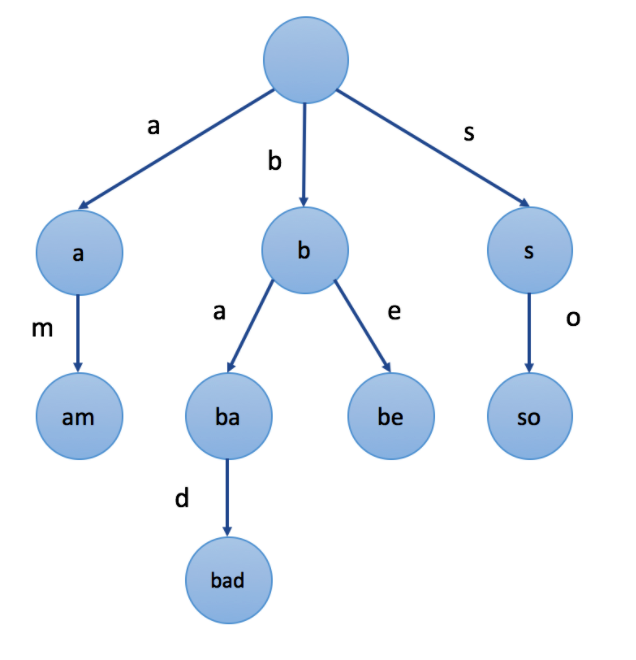
\includegraphics{../static/trie.png}
\caption{Trie}
\end{figure}

    \^{}example of what a \textbf{TRIE} may look like

\begin{itemize}
\tightlist
\item
  notice how root is empty
\item
  all descendants of a node have a common prefix
\item
  widely used in autocomplete, spell checkers
\item
  can represent a trie with an array or a hashmap
\end{itemize}

    This is how you insert into trie. O(N) time

    \begin{figure}
\centering
\includegraphics{../static/insert-trie.gif}
\caption{insert}
\end{figure}

    and how you search in a Trie. O(N) time

    \begin{figure}
\centering
\includegraphics{../static/search-trie.gif}
\caption{search}
\end{figure}

    \textbf{Trie} is also sometimes called \textbf{prefix tree}, it is a
special form \textbf{N-ary tree} (meaning each node can have no more
than \textbf{N} children)

Origin of word \textbf{trie} is from re\textbf{trie}ve

    You use an array or a hashmap to implement a \textbf{Trie}. For example

    \begin{tcolorbox}[breakable, size=fbox, boxrule=1pt, pad at break*=1mm,colback=cellbackground, colframe=cellborder]
\prompt{In}{incolor}{4}{\boxspacing}
\begin{Verbatim}[commandchars=\\\{\}]
\PY{k+kn}{from} \PY{n+nn}{typing} \PY{k+kn}{import} \PY{n}{Tuple}
\PY{k+kn}{import} \PY{n+nn}{json}


\PY{k}{class} \PY{n+nc}{TrieNode}\PY{p}{:}
    \PY{k}{def} \PY{n+nf+fm}{\PYZus{}\PYZus{}init\PYZus{}\PYZus{}}\PY{p}{(}\PY{n+nb+bp}{self}\PY{p}{,} \PY{n}{char}\PY{p}{:} \PY{n+nb}{str}\PY{p}{)}\PY{p}{:}
        \PY{n+nb+bp}{self}\PY{o}{.}\PY{n}{char} \PY{o}{=} \PY{n}{char}
        \PY{n+nb+bp}{self}\PY{o}{.}\PY{n}{children} \PY{o}{=} \PY{p}{[}\PY{p}{]}          \PY{c+c1}{\PYZsh{} using an array to store children}
        \PY{n+nb+bp}{self}\PY{o}{.}\PY{n}{word\PYZus{}finished} \PY{o}{=} \PY{k+kc}{False}  \PY{c+c1}{\PYZsh{} Is it the last character of the word ?}
        \PY{n+nb+bp}{self}\PY{o}{.}\PY{n}{counter} \PY{o}{=} \PY{l+m+mi}{1}            \PY{c+c1}{\PYZsh{} How many times this character appeared in the addition process}

    \PY{c+c1}{\PYZsh{} could have used \PYZus{}\PYZus{}str\PYZus{}\PYZus{} as well. \PYZus{}\PYZus{}repr\PYZus{}\PYZus{} conventional use is to reconstruct}
    \PY{c+c1}{\PYZsh{} the instance of a class given a string. For example, if class Foo has a single}
    \PY{c+c1}{\PYZsh{} attribute bar, and its value is \PYZsq{}bar\PYZsq{}, then \PYZus{}\PYZus{}repr\PYZus{}\PYZus{} would return}
    \PY{c+c1}{\PYZsh{} Foo(bar=\PYZsq{}bar\PYZsq{}). Here we use \PYZus{}\PYZus{}repr\PYZus{}\PYZus{} to help us visualize the Trie}
    \PY{k}{def} \PY{n+nf+fm}{\PYZus{}\PYZus{}repr\PYZus{}\PYZus{}}\PY{p}{(}\PY{n+nb+bp}{self}\PY{p}{)}\PY{p}{:}
        \PY{k}{return} \PY{n}{json}\PY{o}{.}\PY{n}{dumps}\PY{p}{(}\PY{n+nb+bp}{self}\PY{o}{.}\PY{n}{\PYZus{}json}\PY{p}{(}\PY{p}{)}\PY{p}{,} \PY{n}{indent}\PY{o}{=}\PY{l+m+mi}{4}\PY{p}{)}

    \PY{k}{def} \PY{n+nf}{\PYZus{}json}\PY{p}{(}\PY{n+nb+bp}{self}\PY{p}{)}\PY{p}{:}
        \PY{k}{return} \PY{p}{\PYZob{}}
            \PY{l+s+s2}{\PYZdq{}}\PY{l+s+s2}{char}\PY{l+s+s2}{\PYZdq{}}\PY{p}{:} \PY{n+nb+bp}{self}\PY{o}{.}\PY{n}{char}\PY{p}{,}
            \PY{l+s+s2}{\PYZdq{}}\PY{l+s+s2}{children}\PY{l+s+s2}{\PYZdq{}}\PY{p}{:} \PY{p}{[}\PY{n}{child}\PY{o}{.}\PY{n}{\PYZus{}json}\PY{p}{(}\PY{p}{)} \PY{k}{for} \PY{n}{child} \PY{o+ow}{in} \PY{n+nb+bp}{self}\PY{o}{.}\PY{n}{children}\PY{p}{]}\PY{p}{,}
            \PY{l+s+s2}{\PYZdq{}}\PY{l+s+s2}{word\PYZus{}finished}\PY{l+s+s2}{\PYZdq{}}\PY{p}{:} \PY{n+nb+bp}{self}\PY{o}{.}\PY{n}{word\PYZus{}finished}\PY{p}{,}
            \PY{l+s+s2}{\PYZdq{}}\PY{l+s+s2}{counter}\PY{l+s+s2}{\PYZdq{}}\PY{p}{:} \PY{n+nb+bp}{self}\PY{o}{.}\PY{n}{counter}\PY{p}{,}
        \PY{p}{\PYZcb{}}


\PY{c+c1}{\PYZsh{} Adds a word to a TrieNode}
\PY{c+c1}{\PYZsh{} 1. current node is root at start}
\PY{c+c1}{\PYZsh{} 2. for each character in the word}
\PY{c+c1}{\PYZsh{}    \PYZhy{} look for the TrieNode whose value (self.char) == this character}
\PY{c+c1}{\PYZsh{}    \PYZhy{} if can\PYZsq{}t find, create a TrieNode; else traverse down the found TrieNode}
\PY{c+c1}{\PYZsh{}}
\PY{c+c1}{\PYZsh{} Time Complexity of this is O(N * M). Meaning very inefficient}
\PY{c+c1}{\PYZsh{} N \PYZhy{} length of word}
\PY{c+c1}{\PYZsh{} M \PYZhy{} maximum number of children a TrieNode can have (a Trie is a special form N\PYZhy{}ary Trie)}
\PY{c+c1}{\PYZsh{}}
\PY{c+c1}{\PYZsh{} How could we improve the time complexity of this algo?}
\PY{c+c1}{\PYZsh{} We could store pointers to the locations of the nodes separately. For example, given the root (its}
\PY{c+c1}{\PYZsh{} hash, or some sort of key), we can look up the pointer to it in a database that would hold this info}
\PY{c+c1}{\PYZsh{} for us. We can now get the instance of the root TrieNode, what next? We can now use the first character}
\PY{c+c1}{\PYZsh{} of the word as an index, to go to the db to get the pointer to the next TrieNode, and so on.}
\PY{c+c1}{\PYZsh{} You will agree that this is much more efficient. We have paid the price of extra storage in return for}
\PY{c+c1}{\PYZsh{} the greater performance (time complexity)}
\PY{c+c1}{\PYZsh{} Our TrieNode now, would at most take}
\PY{c+c1}{\PYZsh{} Time Complexity O(N)}
\PY{c+c1}{\PYZsh{} with Space Complexity O(L), where L is the total number of TrieNodes (many of TrieNode)}
\PY{c+c1}{\PYZsh{} If you look here: https://eth.wiki/en/fundamentals/patricia\PYZhy{}tree}
\PY{c+c1}{\PYZsh{} then that is exactly how it is done in Ethereum. The only caveat, Ethereum doesn\PYZsq{}t use Tries, at least,}
\PY{c+c1}{\PYZsh{} not the basic prefix tries. Let\PYZsq{}s continue exploring to understand why}
\PY{k}{def} \PY{n+nf}{add}\PY{p}{(}\PY{n}{root}\PY{p}{,} \PY{n}{word}\PY{p}{:} \PY{n+nb}{str}\PY{p}{)}\PY{p}{:}
    \PY{n}{node} \PY{o}{=} \PY{n}{root}
    \PY{k}{for} \PY{n}{char} \PY{o+ow}{in} \PY{n}{word}\PY{p}{:}
        \PY{n}{found\PYZus{}in\PYZus{}child} \PY{o}{=} \PY{k+kc}{False}
        \PY{k}{for} \PY{n}{child} \PY{o+ow}{in} \PY{n}{node}\PY{o}{.}\PY{n}{children}\PY{p}{:}
            \PY{k}{if} \PY{n}{child}\PY{o}{.}\PY{n}{char} \PY{o}{==} \PY{n}{char}\PY{p}{:}
                \PY{n}{child}\PY{o}{.}\PY{n}{counter} \PY{o}{+}\PY{o}{=} \PY{l+m+mi}{1}
                \PY{n}{node} \PY{o}{=} \PY{n}{child}
                \PY{n}{found\PYZus{}in\PYZus{}child} \PY{o}{=} \PY{k+kc}{True}
                \PY{k}{break}

        \PY{k}{if} \PY{o+ow}{not} \PY{n}{found\PYZus{}in\PYZus{}child}\PY{p}{:}
            \PY{n}{new\PYZus{}node} \PY{o}{=} \PY{n}{TrieNode}\PY{p}{(}\PY{n}{char}\PY{p}{)}
            \PY{n}{node}\PY{o}{.}\PY{n}{children}\PY{o}{.}\PY{n}{append}\PY{p}{(}\PY{n}{new\PYZus{}node}\PY{p}{)}
            \PY{n}{node} \PY{o}{=} \PY{n}{new\PYZus{}node}

    \PY{n}{node}\PY{o}{.}\PY{n}{word\PYZus{}finished} \PY{o}{=} \PY{k+kc}{True}


\PY{c+c1}{\PYZsh{} def find\PYZus{}prefix(root, prefix: str) \PYZhy{}\PYZgt{} Tuple[bool, int]:}
\PY{c+c1}{\PYZsh{}     node = root}
\PY{c+c1}{\PYZsh{}     if not root.children:}
\PY{c+c1}{\PYZsh{}         return False, 0}
\PY{c+c1}{\PYZsh{}     for char in prefix:}
\PY{c+c1}{\PYZsh{}         char\PYZus{}not\PYZus{}found = True}
\PY{c+c1}{\PYZsh{}         for child in node.children:}
\PY{c+c1}{\PYZsh{}             if child.char == char:}
\PY{c+c1}{\PYZsh{}                 char\PYZus{}not\PYZus{}found = False}
\PY{c+c1}{\PYZsh{}                 node = child}
\PY{c+c1}{\PYZsh{}                 break}
\PY{c+c1}{\PYZsh{}         if char\PYZus{}not\PYZus{}found:}
\PY{c+c1}{\PYZsh{}             return False, 0}
\PY{c+c1}{\PYZsh{}     return True, node.counter}


\PY{c+c1}{\PYZsh{} print(find\PYZus{}prefix(root, \PYZsq{}hac\PYZsq{}))}
\PY{c+c1}{\PYZsh{} print(find\PYZus{}prefix(root, \PYZsq{}hack\PYZsq{}))}
\PY{c+c1}{\PYZsh{} print(find\PYZus{}prefix(root, \PYZsq{}hackathon\PYZsq{}))}
\PY{c+c1}{\PYZsh{} print(find\PYZus{}prefix(root, \PYZsq{}ha\PYZsq{}))}
\PY{c+c1}{\PYZsh{} print(find\PYZus{}prefix(root, \PYZsq{}hammer\PYZsq{}))}
\end{Verbatim}
\end{tcolorbox}

    \begin{tcolorbox}[breakable, size=fbox, boxrule=1pt, pad at break*=1mm,colback=cellbackground, colframe=cellborder]
\prompt{In}{incolor}{5}{\boxspacing}
\begin{Verbatim}[commandchars=\\\{\}]
\PY{n}{root} \PY{o}{=} \PY{n}{TrieNode}\PY{p}{(}\PY{l+s+s1}{\PYZsq{}}\PY{l+s+s1}{*}\PY{l+s+s1}{\PYZsq{}}\PY{p}{)}
\PY{n}{add}\PY{p}{(}\PY{n}{root}\PY{p}{,} \PY{l+s+s2}{\PYZdq{}}\PY{l+s+s2}{dog}\PY{l+s+s2}{\PYZdq{}}\PY{p}{)}
\PY{n}{add}\PY{p}{(}\PY{n}{root}\PY{p}{,} \PY{l+s+s2}{\PYZdq{}}\PY{l+s+s2}{done}\PY{l+s+s2}{\PYZdq{}}\PY{p}{)}
\PY{n}{add}\PY{p}{(}\PY{n}{root}\PY{p}{,} \PY{l+s+s2}{\PYZdq{}}\PY{l+s+s2}{dope}\PY{l+s+s2}{\PYZdq{}}\PY{p}{)}
\end{Verbatim}
\end{tcolorbox}

    \begin{tcolorbox}[breakable, size=fbox, boxrule=1pt, pad at break*=1mm,colback=cellbackground, colframe=cellborder]
\prompt{In}{incolor}{6}{\boxspacing}
\begin{Verbatim}[commandchars=\\\{\}]
\PY{n}{root}
\end{Verbatim}
\end{tcolorbox}

            \begin{tcolorbox}[breakable, size=fbox, boxrule=.5pt, pad at break*=1mm, opacityfill=0]
\prompt{Out}{outcolor}{6}{\boxspacing}
\begin{Verbatim}[commandchars=\\\{\}]
\{
    "char": "*",
    "children": [
        \{
            "char": "d",
            "children": [
                \{
                    "char": "o",
                    "children": [
                        \{
                            "char": "g",
                            "children": [],
                            "word\_finished": true,
                            "counter": 1
                        \},
                        \{
                            "char": "n",
                            "children": [
                                \{
                                    "char": "e",
                                    "children": [],
                                    "word\_finished": true,
                                    "counter": 1
                                \}
                            ],
                            "word\_finished": false,
                            "counter": 1
                        \},
                        \{
                            "char": "p",
                            "children": [
                                \{
                                    "char": "e",
                                    "children": [],
                                    "word\_finished": true,
                                    "counter": 1
                                \}
                            ],
                            "word\_finished": false,
                            "counter": 1
                        \}
                    ],
                    "word\_finished": false,
                    "counter": 3
                \}
            ],
            "word\_finished": false,
            "counter": 3
        \}
    ],
    "word\_finished": false,
    "counter": 1
\}
\end{Verbatim}
\end{tcolorbox}
        
    \hypertarget{why-dont-we-use-trie-in-ethereum}{%
\subsection{WHY DON'T WE USE TRIE IN
ETHEREUM?}\label{why-dont-we-use-trie-in-ethereum}}

\begin{itemize}
\tightlist
\item
  awful time complexity
\item
  even if improved (like above), wastes space (see radix trie below for
  comparison)
\item
  not useful, because we can't verify the integrity and validity of the
  data
\end{itemize}

    \hypertarget{radix-trie}{%
\section{RADIX TRIE}\label{radix-trie}}

    \begin{figure}
\centering
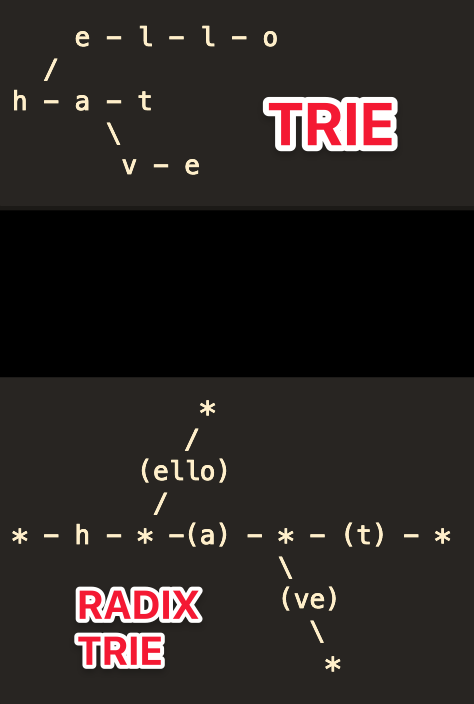
\includegraphics{../static/trie-vs-radix.png}
\caption{trie-vs-radix}
\end{figure}

    \begin{figure}
\centering
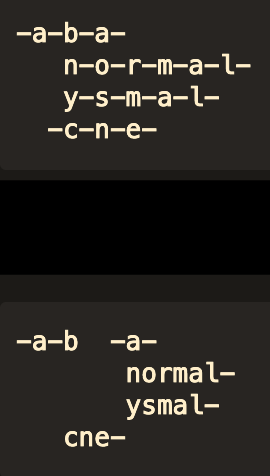
\includegraphics{../static/trie-vs-radix-2.png}
\caption{trie-vs-radix-2}
\end{figure}

    i.e.~the RADIX TRIE uses the space better. So RADIX TRIE is just like
TRIE, but with better space

    \hypertarget{merkle-trie-patricia-trie}{%
\section{Merkle Trie \textbar{} Patricia
Trie}\label{merkle-trie-patricia-trie}}

    \textbf{Just like Radix trie, with an addition of being
cryptographically verifiable}

    \begin{longtable}[]{@{}l@{}}
\toprule
\endhead
\begin{minipage}[t]{0.71\columnwidth}\raggedright
INCOSISTENCY in eth.wiki (I think):\strut
\end{minipage}\tabularnewline
\begin{minipage}[t]{0.71\columnwidth}\raggedright
From: https://eth.wiki/en/fundamentals/patricia-tree\strut
\end{minipage}\tabularnewline
\begin{minipage}[t]{0.71\columnwidth}\raggedright
""" radix tries have one major limitation: they are inefficient. If you
want to store just one (path,value) binding where the path is (in the
case of the ethereum state trie), 64 characters long (number of nibbles
in bytes32), you will need over a kilobyte of extra space to store one
level per character, and each lookup or delete will take the full 64
steps """\strut
\end{minipage}\tabularnewline
\begin{minipage}[t]{0.71\columnwidth}\raggedright
\^{} I believe this explanation is incorrect. It is not radix tries that
have this issue, but tries. Radix tries fix this problem, as we have
seen from the screenshots above. We do not need to create a 17 item
array for each nibble. If we have a single (path, value) binding, then
we can just store path and the value in the very first node after
root\strut
\end{minipage}\tabularnewline
\bottomrule
\end{longtable}

    \textbf{LEAF NODE} - a node that doesn't have children

Merkle Tries are usually implemented as binary tries

Merkle Tries are most useful in:

\begin{enumerate}
\def\labelenumi{(\roman{enumi})}
\tightlist
\item
  distributed systems, for efficient data verification
\end{enumerate}

e.g.~in Git, Tor, Bitcoin ANNNND in Ethereum

\begin{center}\rule{0.5\linewidth}{0.5pt}\end{center}

    \begin{figure}
\centering
\includegraphics{../static/Hash_Tree.png}
\caption{merkle trie}
\end{figure}

    Modified Merkle Trie is Ethereum's optimized Merkle Trie

    \hypertarget{modified-merkle-patricia-trie-merkle-patricia-trie-modified-merkle-trie}{%
\subsection{Modified Merkle Patricia Trie \textbar{} Merkle Patricia
Trie \textbar{} Modified Merkle
Trie}\label{modified-merkle-patricia-trie-merkle-patricia-trie-modified-merkle-trie}}

    Ethereum's data structure is often called Merkle Patricia Trie, without
the Modified prefix

It is ``Modified'' because it has been optimised for Ethereum's needs

For example, in Modified Merkle Patricia Trie, there are three types of
nodes:

\begin{enumerate}
\def\labelenumi{(\roman{enumi})}
\item
  \textbf{branch node}
\item
  \textbf{extension node}
\item
  \textbf{leaf node}
\end{enumerate}

We need these, to primarily make better use of space

    \textbf{MPT} is

\begin{itemize}
\item
  CRYPTOGRAPHICALLY AUTHENTICATED
\item
  can store all (key, value) bindings (we RLP encode the key)
\item
  O(log N) INSERT, LOOKUP, DELETE
\end{itemize}

    \textbf{Note}

Due to the introduction of extension and leaf nodes, we may end up
having to traverse an odd-length remaining path. This introduces a
challenge

    All paths are stored as \texttt{bytes} type, and a single byte is 2
nibbles (2 hex chars). In this setting, how do you distinguish nibble
`1' from a nibble `01'? You can't. Both are represented as
\texttt{\textless{}01\textgreater{}} \texttt{bytes} (you cannot create a
byte from odd-length nibbles)

1 byte = 2 hex

So we must do something about this. We can trivially solve this issue
with flags. We can prefix all the 2-item nodes (leaf and extension) with
the following

    \begin{figure}
\centering
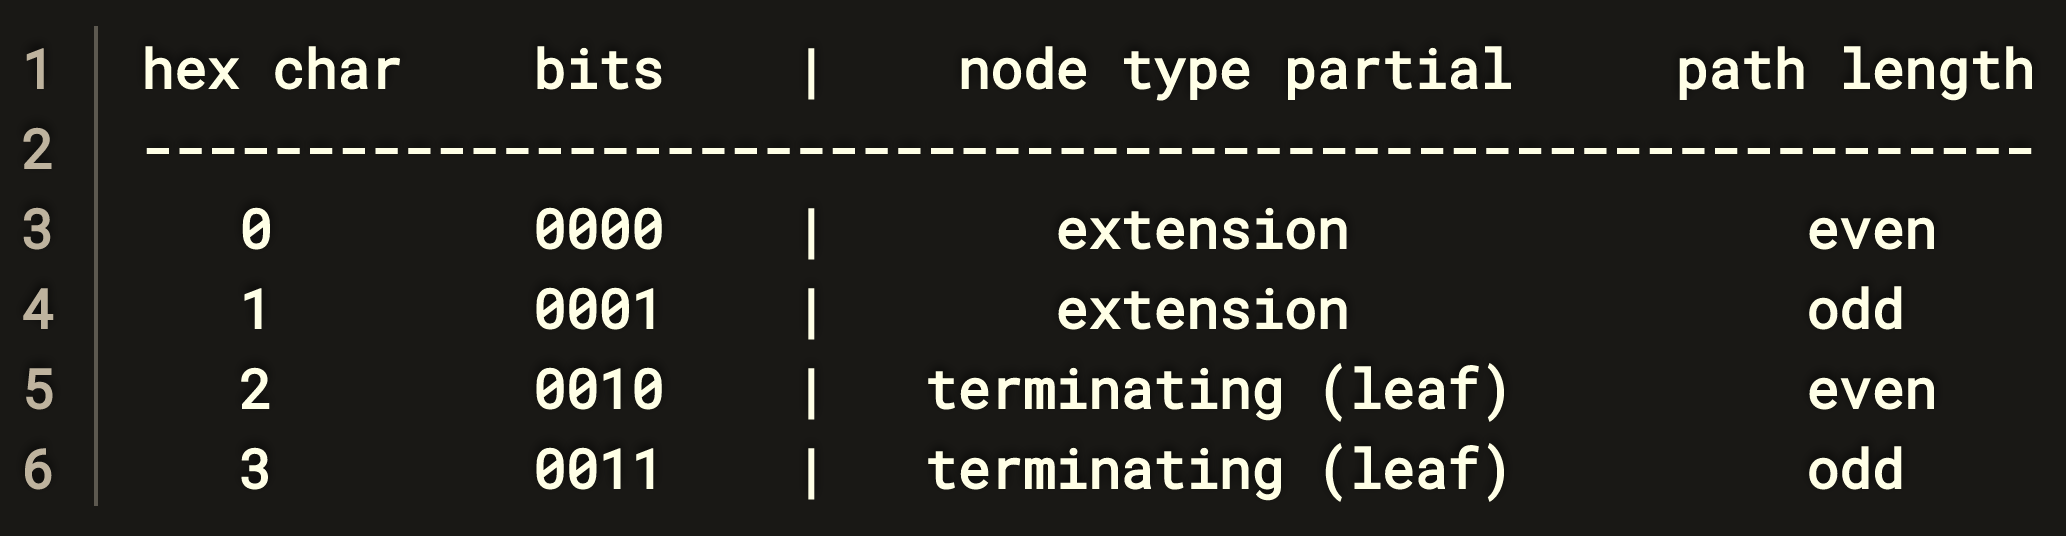
\includegraphics{../static/prefix-flags.png}
\caption{prefix-flags}
\end{figure}

    we do not care about the branch node because it does not contain the
nibble path, and so does not suffer from this problem

    I find it very difficult to understand the Merkle Patricia Trie on
eth.wiki, their \texttt{compact\_encode} function is a bit strange too.
So we will be implementing our own hex prefix algorithm from the yellow
paper. Here is what it should do

    \begin{figure}
\centering
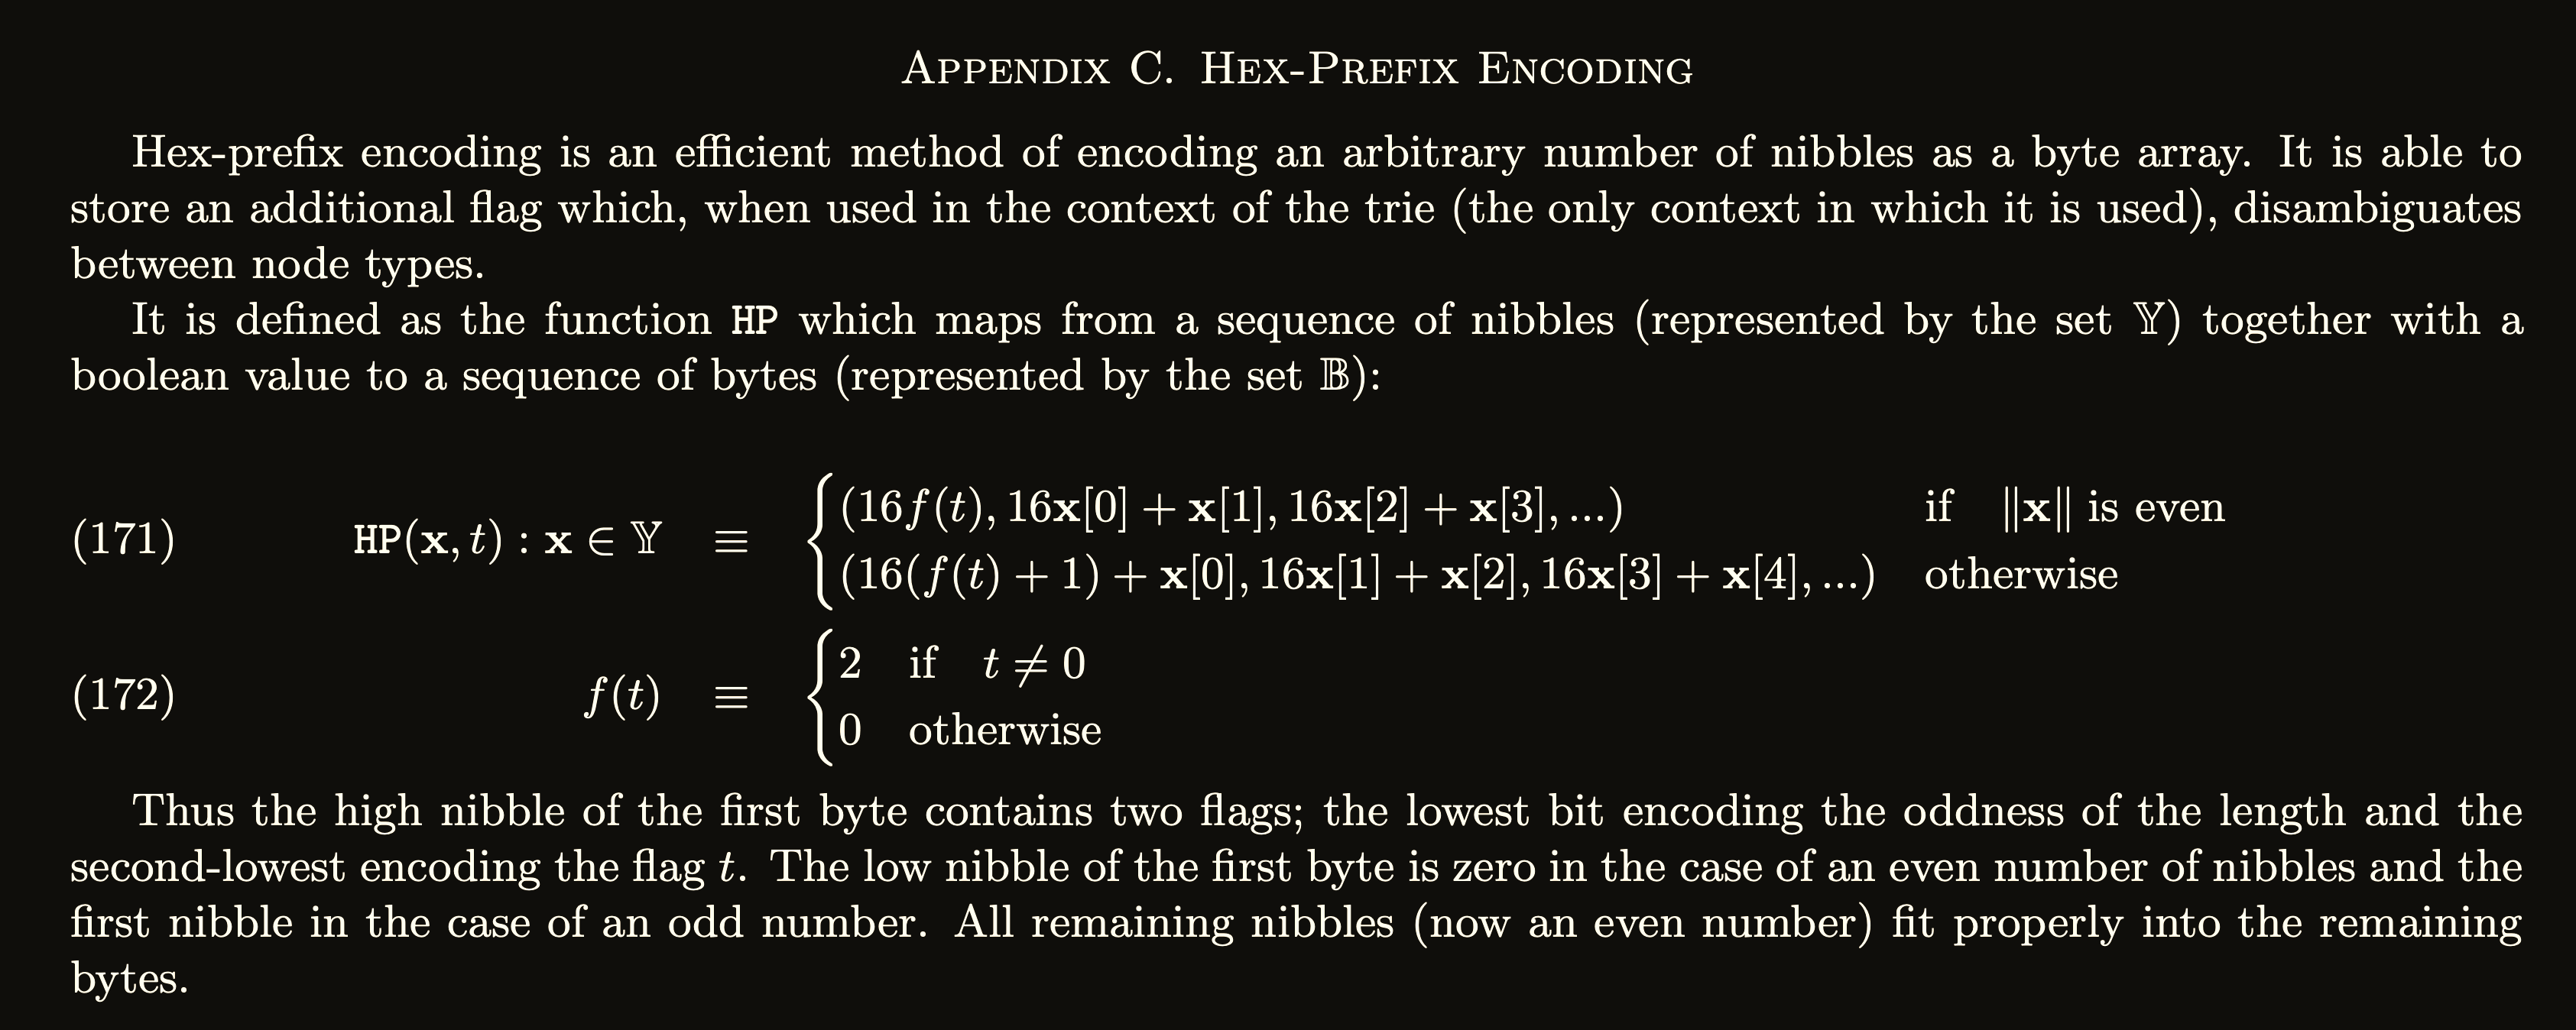
\includegraphics{../static/hex-prefix.png}
\caption{hex-prefix}
\end{figure}

    To be honest with you, even this is a bit confusing. First of all, there
is no definition of what \(t\) is, except for the fact that it is
boolean. We can probably, assume, that \(t\) is the node type (extension
or leaf). Though, it remains to be determined whether extension === True
or leaf === True

Then, \(||x||\) is the notation that is generally used to denote an
\(L_2\) norm (i.e.~the length of the line /vector in Euclidean space),
although, in this particular case, it appears that it is used as the
cardinality of the set, where each x{[}i{]} is the hex character. It is
not clear why we need to do those mathematical operations in any case

    Given the above, let's just look at the most popular client out there:
geth. And see how they do it

    \hypertarget{the-comment-section-before-the-hextocompact-implementation}{%
\paragraph{the comment section before the hexToCompact
implementation:}\label{the-comment-section-before-the-hextocompact-implementation}}

Trie keys are dealt with in three distinct encodings:

KEYBYTES encoding contains the actual key and nothing else. This
encoding is the input to most API functions.

HEX encoding contains one byte for each nibble of the key and an
optional trailing `terminator' byte of value 0x10 which indicates
whether or not the node at the key contains a value. Hex key encoding is
used for nodes loaded in memory because it's convenient to access.

COMPACT encoding is defined by the Ethereum Yellow Paper (it's called
``hex prefix encoding'' there) and contains the bytes of the key and a
flag. The high nibble of the first byte contains the flag; the lowest
bit encoding the oddness of the length and the second-lowest encoding
whether the node at the key is a value node. The low nibble of the first
byte is zero in the case of an even number of nibbles and the first
nibble in the case of an odd number. All remaining nibbles (now an even
number) fit properly into the remaining bytes. Compact encoding is used
for nodes stored on disk.

    \begin{figure}
\centering
\includegraphics{../static/hexToCompact.png}
\caption{hexToCompace}
\end{figure}

    and here is the test for the above function

    \begin{figure}
\centering
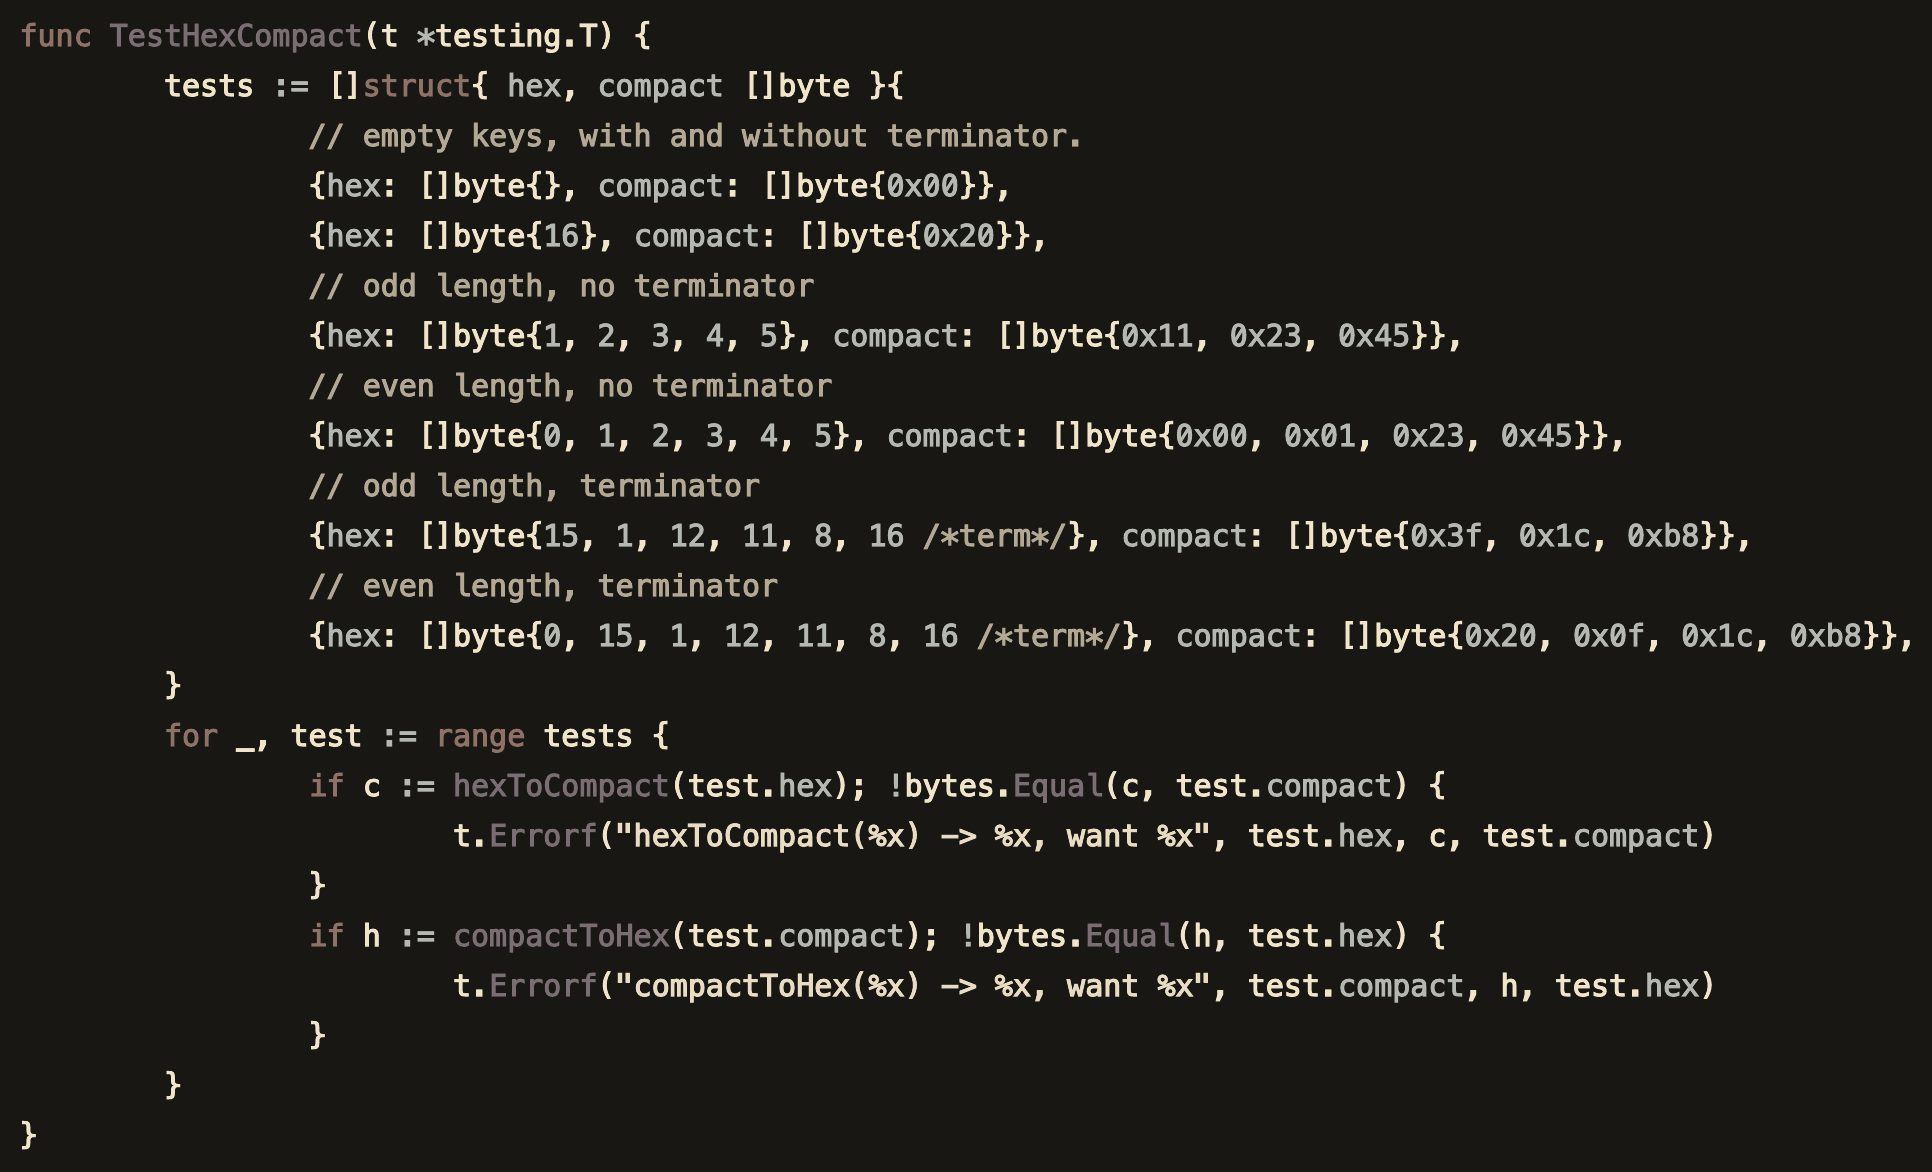
\includegraphics{../static/test-hex-to-compact.png}
\caption{test-hex-to-compact}
\end{figure}

    so, as you can see the distinction between the leaf and extension node
is made via an optional terminator flag that is placed at the end of the
bytearray. From now on, we shall use geth as our source of truth. It
appears to me, that the reason for popularity of geth is perhaps, partly
due to the clarity of the code

    Let's conclude on this note. Perhaps we will dive deeper in the near
future. For now, this knowledge will suffice

    If you are interested, there is a nice utility in ethereum/hexbytes repo
on GitHub. It will nicely format the Python's ugly bytes to hexadecimal
for you, here:

    \begin{tcolorbox}[breakable, size=fbox, boxrule=1pt, pad at break*=1mm,colback=cellbackground, colframe=cellborder]
\prompt{In}{incolor}{87}{\boxspacing}
\begin{Verbatim}[commandchars=\\\{\}]
\PY{n}{HexBytes}\PY{p}{(}\PY{l+s+s2}{\PYZdq{}}\PY{l+s+se}{\PYZbs{}x03}\PY{l+s+se}{\PYZbs{}x08}\PY{l+s+s2}{wf}\PY{l+s+se}{\PYZbs{}xbf}\PY{l+s+s2}{h}\PY{l+s+se}{\PYZbs{}xe7}\PY{l+s+se}{\PYZbs{}x86}\PY{l+s+s2}{q}\PY{l+s+se}{\PYZbs{}xd1}\PY{l+s+se}{\PYZbs{}xea}\PY{l+s+s2}{Cj}\PY{l+s+se}{\PYZbs{}xe0}\PY{l+s+se}{\PYZbs{}x87}\PY{l+s+se}{\PYZbs{}xda}\PY{l+s+s2}{t}\PY{l+s+se}{\PYZbs{}xa1}\PY{l+s+s2}{\PYZsq{}}\PY{l+s+s2}{a}\PY{l+s+se}{\PYZbs{}xda}\PY{l+s+se}{\PYZbs{}xc0}\PY{l+s+se}{\PYZbs{}x01}\PY{l+s+se}{\PYZbs{}x1a}\PY{l+s+se}{\PYZbs{}x9e}\PY{l+s+se}{\PYZbs{}xdd}\PY{l+s+se}{\PYZbs{}xc4}\PY{l+s+se}{\PYZbs{}x90}\PY{l+s+se}{\PYZbs{}x0b}\PY{l+s+se}{\PYZbs{}xf1}\PY{l+s+s2}{\PYZdq{}}\PY{o}{.}\PY{n}{encode}\PY{p}{(}\PY{l+s+s2}{\PYZdq{}}\PY{l+s+s2}{iso\PYZhy{}8859\PYZhy{}1}\PY{l+s+s2}{\PYZdq{}}\PY{p}{)}\PY{p}{)}
\end{Verbatim}
\end{tcolorbox}

            \begin{tcolorbox}[breakable, size=fbox, boxrule=.5pt, pad at break*=1mm, opacityfill=0]
\prompt{Out}{outcolor}{87}{\boxspacing}
\begin{Verbatim}[commandchars=\\\{\}]
HexBytes('0x03087766bf68e78671d1ea436ae087da74a12761dac0011a9eddc4900bf1')
\end{Verbatim}
\end{tcolorbox}
        
    \begin{center}\rule{0.5\linewidth}{0.5pt}\end{center}

\hypertarget{to-sum-up}{%
\section{To sum up}\label{to-sum-up}}

\textbf{Trie} - not very efficient in terms of space and time
complexity. Mostly used in spell checkers and auto-complete

\textbf{Radix Trie} - mostly used in IP routing and associative arrays
implementations

\textbf{Merkle Trie} - cryptographically authenticated data structure,
lets you easily and efficiently check if portions or all of the data has
been tampered with

\textbf{Modified Merkle Trie} - a Merkle Trie modification that is
optimised for Ethereum. Main difference is in the introduction of three
new types of nodes: extension, branch and leaf

\begin{center}\rule{0.5\linewidth}{0.5pt}\end{center}

    \hypertarget{correct-synnonyms}{%
\subsection{Correct synnonyms}\label{correct-synnonyms}}

\textbf{Trie}, prefix trie, digital trie

\textbf{Radix Trie} (sometimes branching factor is specified, for
example Radix 2 Trie. Meaning each node has up to 2 child nodes)

\textbf{Merkle Trie}, Patricia Trie, Hash Trie

\textbf{Modified Merkle Trie}, Modified Merkle Patricia Trie, Merkle
Patricia Trie \textless- ETHEREUM's data structure to store world state

\begin{center}\rule{0.5\linewidth}{0.5pt}\end{center}

    \begin{figure}
\centering
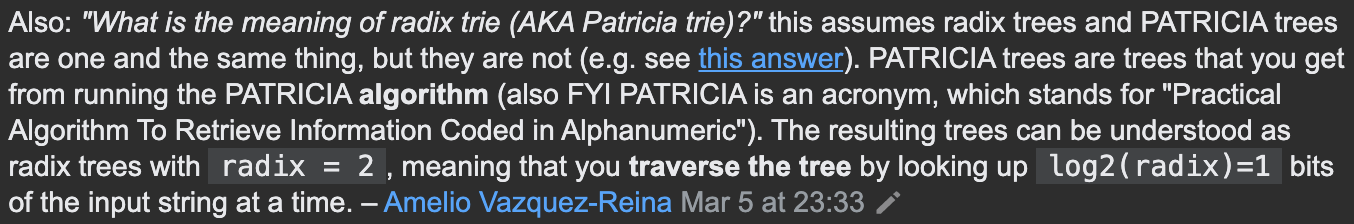
\includegraphics{../static/patricia-is-radix.png}
\caption{patricia-trie-not-radix-trie}
\end{figure}

    source:
https://stackoverflow.com/questions/14708134/what-is-the-difference-between-trie-and-radix-trie-data-structures

    \hypertarget{word-origins}{%
\subsection{Word origins}\label{word-origins}}

\textbf{Trie} - from re\textbf{trie}ve

\textbf{Patricia} - Practical Algorithm To Retrieve Information Coded In
Alphanumeric

\textbf{Radix} - ``In a positional numeral system, the radix or base is
the number of unique digits, including the digit zero, used to represent
numbers'' \textless- from Wikipedia

\textbf{Merkle} - Ralph Merkle patented the Merkle tree in 1979

    \hypertarget{why-modified-merkle-patricia-trie-and-not-xyz-e.g.-pasta-or-yam}{%
\section{Why Modified Merkle Patricia Trie and not XYZ (e.g.~\$PASTA or
\$YAM)?}\label{why-modified-merkle-patricia-trie-and-not-xyz-e.g.-pasta-or-yam}}

\begin{enumerate}
\def\labelenumi{\arabic{enumi}.}
\tightlist
\item
  Cryptographically secure and efficiently verifiable, especially useful
  in the distributed setting
\item
  Optimal insert / lookup / delete time complexities: O(log N)
\item
  Reasonable-ish space complexity
\end{enumerate}

    \hypertarget{better-data-structure-for-ethereum}{%
\section{Better data structure for
Ethereum?}\label{better-data-structure-for-ethereum}}

    I have come across https://arxiv.org/pdf/1909.11590.pdf during my
research, that may present itself to be a worthy substitute

Authors claim 20k TPS\ldots{}

    \begin{tcolorbox}[breakable, size=fbox, boxrule=1pt, pad at break*=1mm,colback=cellbackground, colframe=cellborder]
\prompt{In}{incolor}{ }{\boxspacing}
\begin{Verbatim}[commandchars=\\\{\}]

\end{Verbatim}
\end{tcolorbox}


    % Add a bibliography block to the postdoc
    
    
    
\end{document}
